\chapter*{\centering CHƯƠNG 2. KIẾN TRÚC HỆ THỐNG VÀ TỔ CHỨC MÃ NGUỒN}
\addcontentsline{toc}{chapter}{\textcolor{fitblue}{CHƯƠNG 2. KIẾN TRÚC HỆ THỐNG VÀ TỔ CHỨC MÃ NGUỒN}}

\noindent \indent Dự án được xây dựng theo hai hướng phân rã bổ trợ nhau: phân hệ và phân tầng. Phân hệ dùng để nhóm các thành phần theo chức năng (RenderAPI, GameLogic, ScreenModules, SystemModules, ApplicationTypes, Asset), từ đó cô lập trách nhiệm, giảm phụ thuộc chéo và giúp mở rộng từng mảng độc lập. Phân tầng là cách tổ chức theo luồng xử lý (hiển thị, logic, hệ thống), làm rõ ranh giới dữ liệu đi qua các tầng và kiểm soát chiều phụ thuộc từ trên xuống. Nhờ kết hợp cả hai, mã nguồn vừa có cấu trúc rõ ràng ở cấp thư mục/chức năng, vừa có kỷ luật kiến trúc ở cấp luồng xử lý, giúp dễ đọc, dễ gỡ lỗi và thuận tiện mở rộng.

\section*{2.1. Kiến trúc phân tầng}
\addcontentsline{toc}{section}{\textcolor{black}{2.1. Kiến trúc phân tầng}}

\noindent \indent Kiến trúc tổng thể của hệ thống được chia thành ba tầng chính, hoạt động phối hợp thông qua một bộ điều phối trung tâm tại lớp màn hình.

\subsection*{2.1.1. Render Layer và Logic Layer}
\addcontentsline{toc}{subsection}{\textcolor{black}{2.1.1. Render Layer và Logic Layer}}

\noindent \indent Đây là hai tầng quan trọng nhất, đảm nhiệm vai trò hiển thị và xử lý "linh hồn" của trò chơi:

\begin{itemize}
    \item \textbf{Render Layer (Tầng hiển thị - Thư mục RenderAPI):}
    \begin{itemize}
        \item \textit{Vai trò:} Chịu trách nhiệm vẽ toàn bộ các thành phần hình ảnh lên màn hình bằng thư viện GDI+.
        \item \textit{Thành phần cốt lõi:} Các mô-đun như \texttt{Renderer} (quản lý vùng đệm), \\ \texttt{UIComponents} (vẽ các thành phần giao diện, Pixel Art) và \texttt{UIScaler} (tính toán tỷ lệ màn hình động).
        \item \textit{Kỹ thuật đặc trưng:} Sử dụng hệ thống bộ nhớ đệm để lưu trữ các đối tượng đồ họa nặng (Bitmap, Brush), giúp tốc độ phản hồi đồ họa cực nhanh và mượt mà. Tầng này chỉ nhận dữ liệu thô và thực hiện việc vẽ, không can thiệp vào logic thắng thua.
    \end{itemize}

    \item \textbf{Logic Layer (Tầng xử lý - Thư mục GameLogic):}
    \begin{itemize}
        \item \textit{Vai trò:} Đảm nhiệm việc kiểm soát luật chơi, trạng thái bàn cờ và bộ não trí tuệ nhân tạo.
        \item \textit{Thành phần cốt lõi:} \texttt{GameRules} (kiểm tra điều kiện thắng), \texttt{GameEngine} (đầu não điều phối trận đấu) và \texttt{BotAI} (xử lý thuật toán tìm kiếm nước đi).
        \item \textit{Đặc điểm:} Tách biệt hoàn toàn với môi trường đồ họa. Tầng Logic làm việc trực tiếp trên các cấu hình dữ liệu và ma trận trạng thái, cho phép hệ thống tính toán hàng triệu trạng thái mà không bị ảnh hưởng bởi tốc độ render của giao diện.
    \end{itemize}
\end{itemize}

\subsection*{2.1.2. System Layer: Tài nguyên, cấu hình và thời gian}
\addcontentsline{toc}{subsection}{\textcolor{black}{2.1.2. System Layer: Tài nguyên, cấu hình và thời gian}}

\noindent \indent Tầng hệ thống (Thư mục SystemModules) đóng vai trò là "hậu cần", cung cấp các dịch vụ nền tảng cho toàn bộ ứng dụng:

\begin{itemize}
    \item \textbf{Quản lý Tài nguyên và Đa ngôn ngữ (Localization):}
    \begin{itemize}
        \item Mô-đun \texttt{Localization} chịu trách nhiệm tải và ánh xạ các chuỗi văn bản từ tệp tin bên ngoài vào ứng dụng. Điều này cho phép chuyển đổi ngôn ngữ (Vietnamese/English) ngay lập tức mà không cần biên dịch lại mã nguồn.
    \end{itemize}

    \item \textbf{Hệ thống cấu hình (ConfigLoader):}
    \begin{itemize}
        \item Sử dụng tệp \texttt{config.ini} để lưu trữ các tùy chỉnh của người dùng như âm lượng, ngôn ngữ, trạng thái bật/tắt nhạc nền. Cơ chế này giúp trò chơi "ghi nhớ" được trạng thái của người chơi qua các lần khởi động khác nhau.
    \end{itemize}

    \item \textbf{Hệ thống Âm thanh (AudioSystem):}
    \begin{itemize}
        \item Đây là một dịch vụ đặc biệt được vận hành theo cơ chế không đồng bộ. Âm thanh được quản lý bởi một luồng tách biệt, giúp các hiệu ứng tiếng vang, nhạc nền hay tiếng hò reo của khán giả có thể phát ra liên tục mà không làm gián đoạn luồng xử lý nước đi của người chơi.
    \end{itemize}

    \item \textbf{Quản lý Thời gian (TimeSystem):}
    \begin{itemize}
        \item Sử dụng thư viện \texttt{chrono} để tính toán chính xác thời gian đếm ngược và tổng thời lượng trận đấu. Hệ thống đảm bảo sự công bằng tuyệt đối trong thi đấu, đặc biệt là khi áp dụng các ràng buộc về thời gian suy nghĩ cho mỗi tuyển thủ.
    \end{itemize}
\end{itemize}

\section*{2.2. Luồng xử lý sự kiện}
\addcontentsline{toc}{section}{\textcolor{black}{2.2. Luồng xử lý sự kiện}}

\noindent \indent Để đảm bảo hiệu năng và sự mượt mà trong các thao tác tương tác, hệ thống ứng dụng một cơ chế vận hành theo thời gian thực thay vì mô hình hướng sự kiện thụ động thông thường.

\subsection*{2.2.1. Vòng lặp trò chơi và Thời gian sai lệch}
\addcontentsline{toc}{subsection}{\textcolor{black}{2.2.1. Vòng lặp trò chơi và Thời gian sai lệch}}

\begin{itemize}
    \item \textbf{Vòng lặp trò chơi:} Tại tệp hệ thống chính (\texttt{main.cpp}), ứng dụng sử dụng cơ chế kiểm tra thông điệp không chặn thông qua hàm \texttt{PeekMessage}. Điều này cho phép ứng dụng liên tục thực hiện các tác vụ cập nhật logic và dựng hình ngay cả khi không có tác động từ người dùng.
    \item \textbf{Thời gian sai lệch:} Để đảm bảo các hiệu ứng chuyển động và hoạt cảnh diễn ra với tốc độ đồng nhất trên mọi cấu hình máy tính, hệ thống sử dụng thư viện \texttt{chrono} để tính toán chính xác khoảng thời gian giữa hai khung hình liên tiếp. Chỉ số này được dùng để nhân với vận tốc của các hiệu ứng (như xung nhịp của bộ đệm, hiệu ứng sóng rung), giúp trò chơi vận hành ổn định tại mức khung hình mục tiêu là 60 FPS.
\end{itemize}

\subsection*{2.2.2. Kỹ thuật vùng đệm kép chống nhấp nháy}
\addcontentsline{toc}{subsection}{\textcolor{black}{2.2.2. Kỹ thuật vùng đệm kép chống nhấp nháy}}

\noindent \indent Nhược điểm của việc dựng hình trực tiếp lên màn hình trong Windows là hiện tượng nhấp nháy do quá trình xóa và vẽ lại diễn ra liên tục. Dự án giải quyết triệt để vấn đề này bằng kỹ thuật vùng đệm kép:

\begin{itemize}
    \item \textbf{Cấu trúc vùng đệm:} Toàn bộ quá trình vẽ từ thư viện GDI+ được thực hiện lên một ngữ cảnh thiết bị ảo trong bộ nhớ (Back Buffer) thay vì trực tiếp lên cửa sổ.
    \item \textbf{Cơ chế hoán đổi:} Chỉ khi tất cả các thành phần đồ họa (bàn cờ, quân cờ, hiệu ứng) đã được vẽ hoàn tất lên vùng đệm, hệ thống mới thực hiện một lệnh sao chép khối lượng lớn (\texttt{BitBlt}) duy nhất để đẩy toàn bộ hình ảnh lên màn hình. 
    \item \textbf{Tối ưu hóa:} Ứng dụng can thiệp vào sự kiện xóa nền hệ thống để ngăn chặn Windows tự ý xóa màn hình trước mỗi khung hình, từ đó tạo ra trải nghiệm hình ảnh cực kỳ ổn định và không có độ trễ.
\end{itemize}

\subsection*{2.2.3. Sơ đồ kiến trúc hệ thống}
\addcontentsline{toc}{subsection}{\textcolor{black}{2.2.3. Biểu đồ phân rã kiến trúc hệ thống}}

\noindent \indent Dưới đây là sơ đồ chi tiết về mối liên kết giữa các mô-đun trong hệ thống. Kiến trúc được thiết kế theo mô hình "Trung tâm trạng thái", nơi thông tin về trạng thái trận đấu (\texttt{PlayState}) được chia sẻ giữa các tầng xử lý và tầng hiển thị:

\begin{figure}[H]
    \centering
    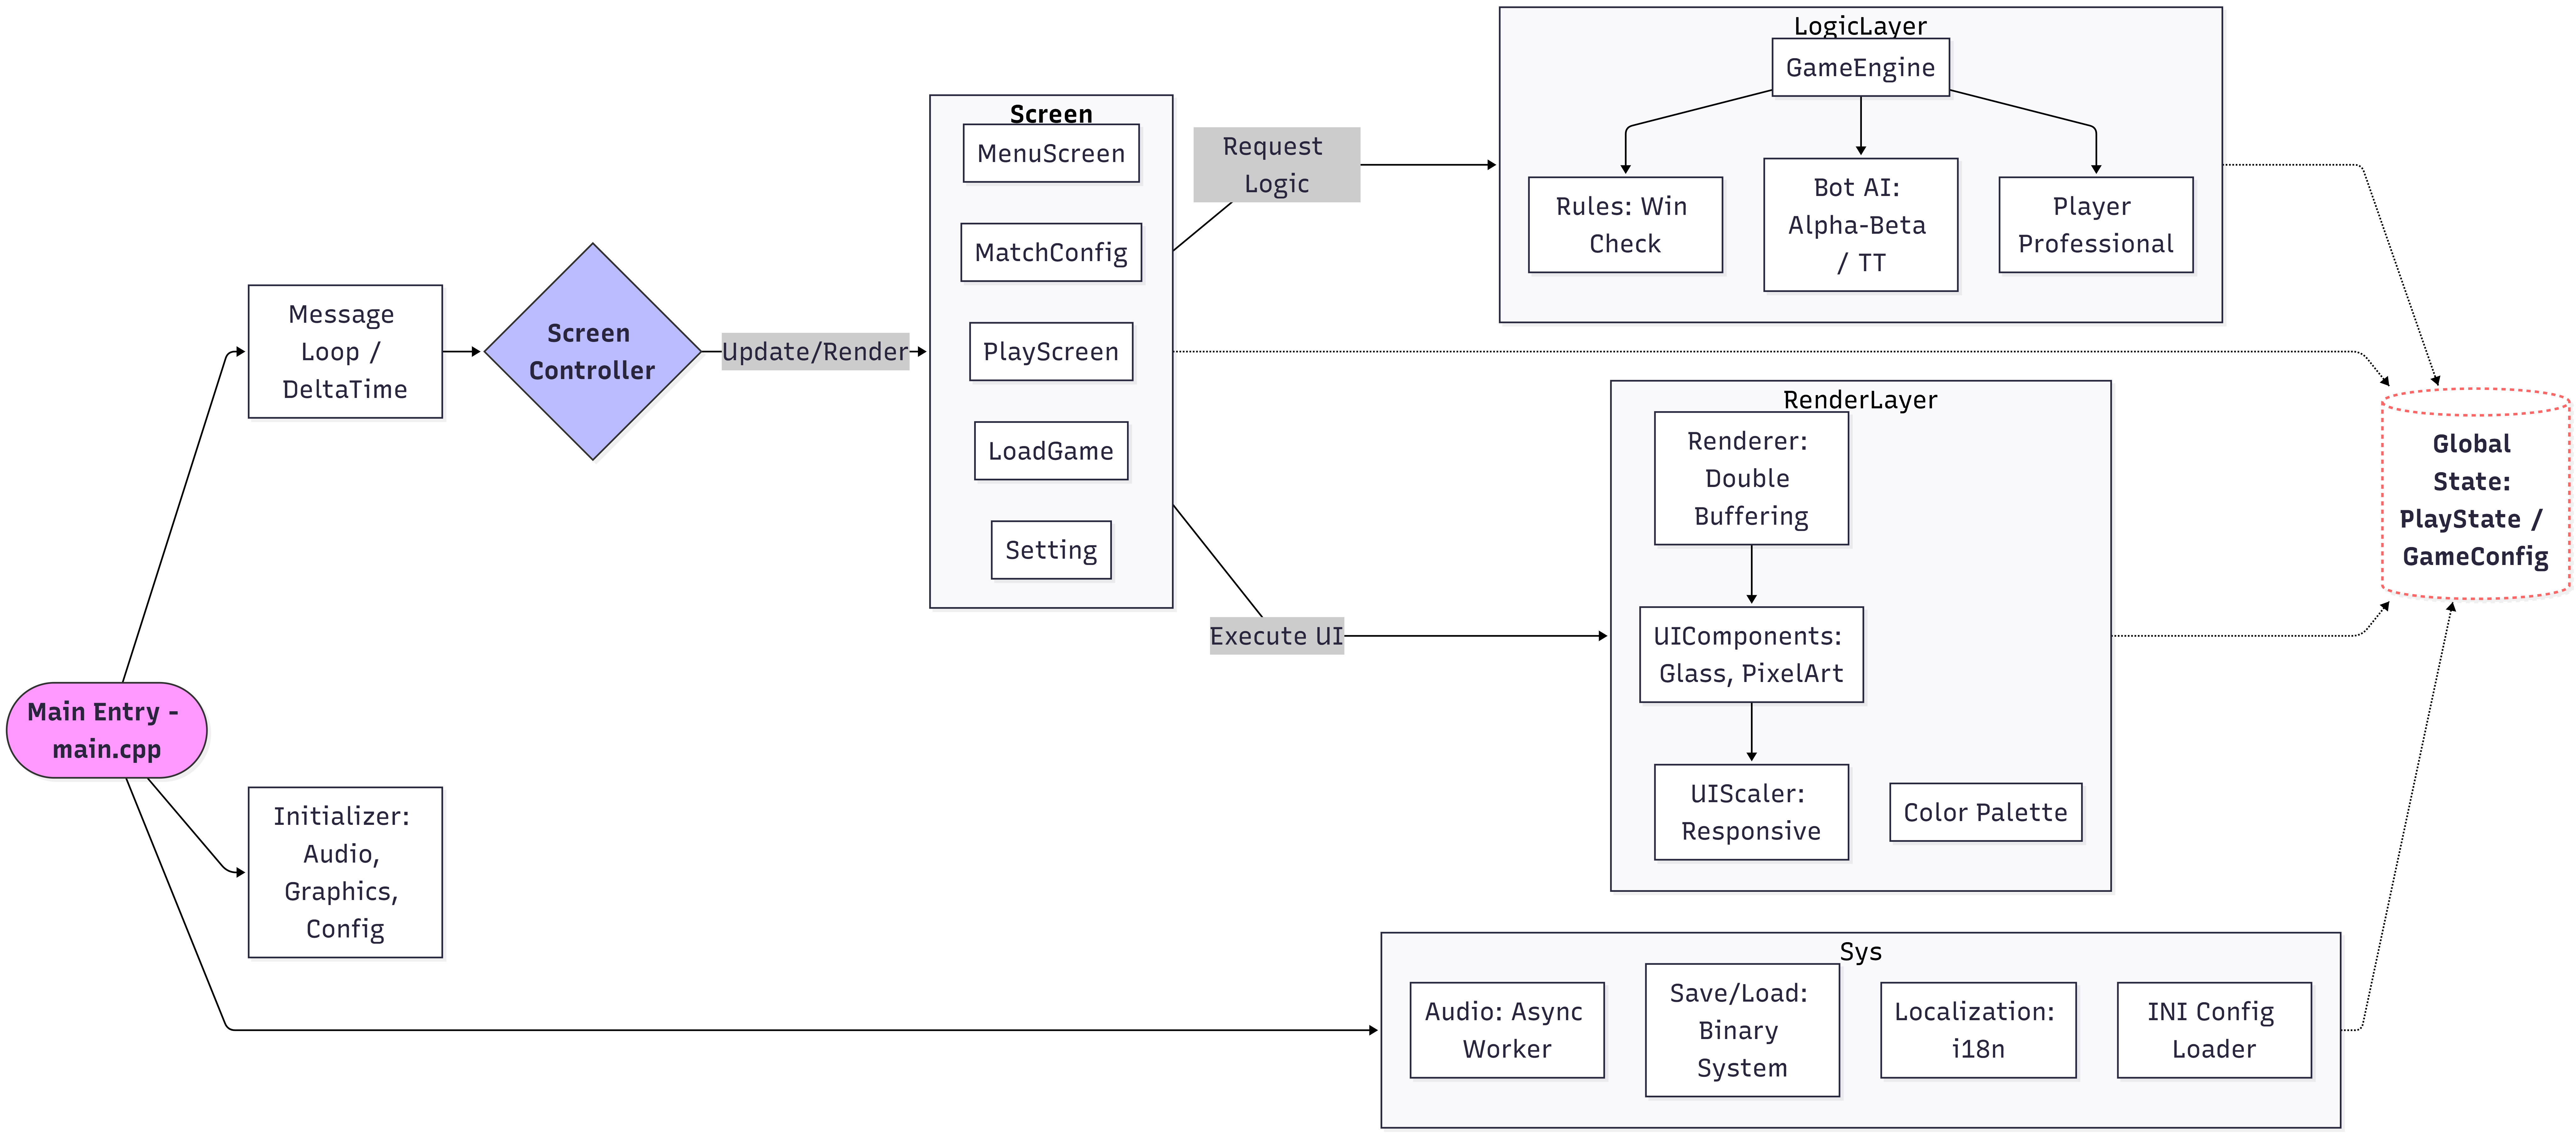
\includegraphics[width=1.4\linewidth, angle=90]{images/uml.png}
    \caption*{Hình 2.1: Sơ đồ kiến trúc hệ thống}
    \addcontentsline{lof}{figure}{Hình 2.1: Sơ đồ kiến trúc hệ thống}
\end{figure}

\textbf{Diễn giải chi tiết các mối quan hệ:}
\begin{itemize}
    \item \textbf{Luồng khởi tạo và vòng lặp chính:} Từ \texttt{main.cpp}, khối khởi tạo nạp Audio/Graphics/Config, sau đó đi vào \textit{Message Loop/DeltaTime}. Nhịp cập nhật này là nguồn kích hoạt cho \textit{Screen Controller}.
    \item \textbf{Tầng điều phối (Screen Controller):} Bộ điều phối chọn màn hình hiện tại (\texttt{MenuScreen}, \texttt{MatchConfig}, \texttt{PlayScreen}, \texttt{LoadGame}, \texttt{Setting}) và gọi \textit{Update/Render}. Khi cần xử lý nước đi hoặc luật, nó gửi \textit{Request Logic} sang \\ \texttt{GameEngine}.
    \item \textbf{LogicLayer:} \texttt{GameEngine} điều phối luật và lượt chơi, gọi \texttt{GameRules} để kiểm tra thắng, dùng \texttt{BotAI} (Alpha-Beta/TT) cho PvE và \texttt{PlayerEngineer} để xử lý thao tác người chơi. Tầng này chỉ làm việc với dữ liệu bàn cờ/trạng thái.
    \item \textbf{RenderLayer:} \texttt{Renderer} dựng khung hình bằng double buffering, \texttt{UIComponents} vẽ Glass/PixelArt, \texttt{UIScaler} đảm bảo responsive, và \texttt{Colours} cung cấp bảng màu đồng nhất.
    \item \textbf{Sys:} Các dịch vụ nền gồm Audio Async Worker, Save/Load Binary, Localization (i18n) và INI Config Loader, được các màn hình và logic gọi theo nhu cầu.
    \item \textbf{Global State:} \texttt{PlayState} và \texttt{GameConfig} là nguồn dữ liệu trung tâm. Logic cập nhật, Render đọc để vẽ, còn Sys đọc/ghi khi lưu/tải hoặc nạp cấu hình, bảo đảm tính nhất quán giữa các tầng.
\end{itemize}


\subsection*{2.2.4. Sơ đồ luồng chương trình}
\addcontentsline{toc}{subsection}{\textcolor{black}{2.2.4. Sơ đồ luồng chương trình}}

\noindent \indent Sơ đồ luồng dưới đây mô tả quá trình từ khi khởi chạy ứng dụng, điều hướng qua các màn hình chức năng cho đến khi kết thúc một vòng đời của trận đấu và thoát chương trình:

\begin{figure}[H]
    \centering
    \includegraphics[width=0.9\linewidth]{images/uml2.png}
    \caption*{Hình 2.2: Sơ đồ luồng chương trình}
    \addcontentsline{lof}{figure}{Hình 2.2: Sơ đồ luồng chương trình}
\end{figure}

\textbf{Mô tả các nút thắt quyết định:}

\begin{itemize}
    \item \textbf{Khởi tạo hệ thống:} Bắt đầu \textrightarrow{} khởi tạo GDI+, Audio, Config. Sau khi sẵn sàng, chương trình chuyển vào luồng điều hướng chính.
    \item \textbf{Điều hướng từ Màn hình chính:} 
    \begin{itemize}
        \item \textit{Chơi} \textrightarrow{} Thiết lập trận đấu \textrightarrow{} Màn hình Play (bắt đầu trận).
        \item \textit{Tải trận} \textrightarrow{} Danh sách bản lưu \textrightarrow{} Chọn slot \textrightarrow{} Xác nhận \textrightarrow{} Màn hình Play.
        \item \textit{Cài đặt} \textrightarrow{} Tùy chỉnh âm thanh/ngôn ngữ.
        \item \textit{Hướng dẫn/Thông tin} \textrightarrow{} Xem tài liệu/giới thiệu.
        \item \textit{Thoát} \textrightarrow{} Giải phóng tài nguyên và kết thúc.
    \end{itemize}
    \item \textbf{Vòng lặp trận đấu (Match Loop):} Màn hình Play nhận input di chuyển/đặt quân \textrightarrow{} logic xử lý (đánh quân hoặc AI tính toán) \textrightarrow{} kiểm tra thắng/hòa. Nếu \textit{chưa} kết thúc, quay lại vòng lặp; nếu \textit{kết thúc ván}, chuyển sang Bảng tổng kết.
    \item \textbf{Menu tạm và Lưu:} Trong khi chơi, nhấn \textit{ESC} mở Menu tạm, cho phép tiếp tục, lưu, hoặc thoát về màn hình chính. Lưu sẽ ghi \texttt{PlayState} ra file để có thể tải lại ở lần sau.
    \item \textbf{Tổng kết và điều hướng sau ván:} Bảng tổng kết ván đấu cho phép lưu, chơi ván tiếp theo (quay lại Match Loop), hoặc trở về Màn hình chính/thoát.
\end{itemize}

\section*{2.3. Cấu trúc thư mục và phân hệ}
\addcontentsline{toc}{section}{\textcolor{black}{2.3. Cấu trúc thư mục và phân hệ}}

\noindent \indent Dự án được tổ chức theo cấu trúc phân rã chức năng nghiêm ngặt, giúp việc quản lý hàng chục tệp tin mã nguồn trở nên khoa học và tránh hiện tượng chồng chéo định nghĩa.

\noindent \indent Cấu trúc thư mục tổng quát của mã nguồn được thể hiện như sau:

{\small
\begin{verbatim}
src/
|---- ApplicationTypes/
|     |---- GameConfig.h
|     |---- GameConstants.h
|     |---- GameState.h
|     |---- PlayState.h
|---- GameLogic/
|     |---- BotAI.cpp
|     |---- BotAI.h
|     |---- GameEngine.cpp
|     |---- GameEngine.h
|     |---- GameRules.cpp
|     |---- GameRules.h
|     |---- PlayerEngineer.cpp
|     |---- PlayerEngineer.h
|---- RenderAPI/
|     |---- Colours.cpp
|     |---- Colours.h
|     |---- Renderer.cpp
|     |---- Renderer.h
|     |---- UIComponents.cpp
|     |---- UIComponents.h
|     |---- UIScaler.cpp
|     |---- UIScaler.h
|---- ScreenModules/
|     |---- AboutScreen.cpp
|     |---- AboutScreen.h
|     |---- GuildScreen.cpp
|     |---- GuildScreen.h
|     |---- LoadGameScreen.cpp
|     |---- LoadGameScreen.h
|     |---- MatchConfigScreen.cpp
|     |---- MatchConfigScreen.h
|     |---- MenuScreen.cpp
|     |---- MenuScreen.h
|     |---- PlayScreen.cpp
|     |---- PlayScreen.h
|     |---- SettingScreen.cpp
|     |---- SettingScreen.h
|---- SystemModules/
|     |---- AudioSystem.cpp
|     |---- AudioSystem.h
|     |---- ConfigLoader.cpp
|     |---- ConfigLoader.h
|     |---- Localization.cpp
|     |---- Localization.h
|     |---- SaveLoadSystem.cpp
|     |---- SaveLoadSystem.h
|     |---- TimeSystem.cpp
|     |---- TimeSystem.h
|---- Asset/
|     |---- config.ini
|     |---- audio/
|     |---- font/
|     |---- lang/
|     |---- models/
|     |---- save/
|---- main.cpp
|---- src.sln
|---- src.vcxproj
|---- src.vcxproj.filters
\end{verbatim}
}

\subsection*{2.3.1. Chi tiết các phân hệ: RenderAPI, GameLogic, ScreenModules và SystemModules}
\addcontentsline{toc}{subsection}{\textcolor{black}{2.3.1. Chi tiết các phân hệ}}

\noindent \indent Mã nguồn và tài nguyên được chia thành 6 thư mục cốt lõi, mỗi thư mục đảm nhiệm một vai trò chuyên biệt trong vòng đời của ứng dụng. Dưới đây là mô tả đầy đủ theo từng phân hệ, nêu rõ trách nhiệm, phạm vi dữ liệu và các mô-đun chính:

\begin{itemize}
    \item \textbf{Phân hệ ApplicationTypes (Nền tảng dữ liệu):}
    Đây là nơi định nghĩa các kiểu dữ liệu và hằng số dùng chung cho toàn bộ dự án, làm "hợp đồng dữ liệu" giữa các tầng. Các tệp tiêu biểu gồm:
    \begin{itemize}
        \item \texttt{GameConfig.h}: lưu cấu hình trận đấu (chế độ chơi, kích thước bàn cờ, thời gian, âm lượng) để các phân hệ khác đọc thống nhất.
        \item \texttt{GameConstants.h}: tập hợp các hằng số hệ thống (kích thước ô, giới hạn mảng, mã trạng thái) nhằm tránh rải rác magic number.
        \item \texttt{GameState.h}: định nghĩa trạng thái tổng quát của ứng dụng và trận đấu (ví dụ: đang ở menu, đang chơi, đang tổng kết).
        \item \texttt{PlayState.h}: cấu trúc trung tâm lưu trạng thái bàn cờ, lượt chơi, lịch sử nước đi, thông số người chơi/AI.
    \end{itemize}
    Việc tập trung dữ liệu tại đây giúp đảm bảo tính nhất quán khi các phân hệ khác cùng truy cập và cập nhật.

    \item \textbf{Phân hệ RenderAPI (Thư viện đồ họa nội bộ):}
    Đóng vai trò là lớp vỏ bọc cho GDI+, cung cấp các công cụ vẽ bậc cao và nhất quán giao diện:
    \begin{itemize}
        \item \texttt{Colours}: quản lý bảng màu, đảm bảo toàn bộ giao diện dùng cùng hệ màu (nút, nền, hiệu ứng).
        \item \texttt{Renderer}: khởi tạo ngữ cảnh đồ họa, quản lý back buffer và thực hiện quy trình vẽ khung hình.
        \item \texttt{UIComponents}: dựng các thành phần giao diện (bàn cờ, quân cờ, nút) từ dữ liệu mô tả.
        \item \texttt{UIScaler}: tính toán tỷ lệ và chuyển đổi tọa độ nhằm hỗ trợ đa độ phân giải và tỷ lệ màn hình.
    \end{itemize}
    Tầng này chỉ nhận dữ liệu đã được chuẩn hóa và không tự ý thay đổi logic trận đấu.

    \item \textbf{Phân hệ GameLogic (Đầu não xử lý):}
    Tập trung vào quy tắc, điều phối trận đấu và trí tuệ nhân tạo:
    \begin{itemize}
        \item \texttt{GameEngine}: điều phối vòng đời trận đấu, xử lý đặt quân, chuyển lượt, kiểm soát trạng thái và lịch sử nước đi.
        \item \texttt{GameRules}: kiểm tra điều kiện thắng, hòa, hợp lệ nước đi theo hàng ngang, dọc, chéo.
        \item \texttt{BotAI}: tính toán nước đi tối ưu cho chế độ PvE, tách biệt khỏi phần đồ họa.
        \item \texttt{PlayerEngineer}: xử lý thao tác người chơi và chuyển dữ liệu đầu vào thành nước đi trước khi chuyển sang \texttt{GameEngine}.
    \end{itemize}
    Mọi xử lý trong phân hệ này chỉ làm việc với dữ liệu thuần (ma trận bàn cờ, trạng thái), không phụ thuộc GDI+.

    \item \textbf{Phân hệ ScreenModules (Quản lý màn hình):}
    Mỗi tệp trong thư mục này tương ứng một màn hình cụ thể, chịu trách nhiệm xử lý input, điều hướng và cập nhật trạng thái hiển thị:
    \begin{itemize}
        \item \texttt{MenuScreen}: màn hình chính, điều hướng đến các chế độ chơi và thiết lập.
        \item \texttt{PlayScreen}: màn hình trận đấu, kết nối trực tiếp với \texttt{GameEngine} và \texttt{Renderer}.
        \item \texttt{MatchConfigScreen}: cấu hình trận đấu (chế độ, nhân vật, luật chơi).
        \item \texttt{LoadGameScreen}: tải trận đã lưu, khôi phục \texttt{PlayState}.
        \item \texttt{SettingScreen}: điều chỉnh âm lượng, ngôn ngữ, tùy chọn hiển thị.
        \item \texttt{AboutScreen} và \texttt{GuildScreen}: các màn hình thông tin/bảng thành tích.
    \end{itemize}
    Cách tổ chức này giúp mỗi màn hình có vòng đời rõ ràng, tránh chồng chéo xử lý.

    \item \textbf{Phân hệ SystemModules (Dịch vụ nền):}
    Cung cấp các dịch vụ hỗ trợ cho toàn ứng dụng:
    \begin{itemize}
        \item \texttt{AudioSystem}: quản lý âm thanh đa luồng, phát nhạc nền và hiệu ứng.
        \item \texttt{ConfigLoader}: tải và lưu cấu hình người dùng từ \texttt{config.ini}.
        \item \texttt{Localization}: nạp và ánh xạ chuỗi đa ngôn ngữ từ tệp tài nguyên.
        \item \texttt{SaveLoadSystem}: lưu/khôi phục \texttt{PlayState} xuống ổ đĩa.
        \item \texttt{TimeSystem}: cung cấp bộ đếm thời gian và đo độ trễ khung hình.
    \end{itemize}
    Các dịch vụ này độc lập với logic trận đấu và được gọi theo nhu cầu của các màn hình.

    \item \textbf{Phân hệ Asset (Tài nguyên dữ liệu):}
    Lưu trữ toàn bộ tài nguyên đầu vào của trò chơi, tách biệt khỏi mã nguồn để dễ cập nhật:
    \begin{itemize}
        \item \texttt{config.ini}: cấu hình người dùng và thiết lập mặc định.
        \item \texttt{audio/}: tệp nhạc nền và hiệu ứng âm thanh.
        \item \texttt{font/}: phông chữ hiển thị trong giao diện.
        \item \texttt{lang/}: tệp ngôn ngữ (Việt/Anh) dùng cho \texttt{Localization}.
        \item \texttt{models/}: dữ liệu pixel art, hình nền, vật thể.
        \item \texttt{save/}: dữ liệu lưu trận và lịch sử chơi.
    \end{itemize}
    Thư mục này giúp tách biệt nội dung và logic, cho phép thay đổi tài nguyên mà không cần biên dịch lại.
\end{itemize}

\subsection*{2.3.2. Quy ước Header, Cấu trúc dữ liệu và Đóng gói dữ liệu}
\addcontentsline{toc}{subsection}{\textcolor{black}{2.3.2. Quy ước Header, Cấu trúc dữ liệu và Đóng gói dữ liệu}}

\noindent \indent Để duy trì tính ổn định của mã nguồn, dự án áp dụng các quy chuẩn lập trình đồng bộ, đảm bảo khả năng mở rộng và giảm lỗi phát sinh khi nhiều mô-đun cùng phát triển:

\begin{itemize}
    \item \textbf{Quy ước tệp tiêu đề (Header Guards):}
    Tất cả các tệp \texttt{.h} đều dùng \texttt{\#ifndef / \#define / \#endif} để chống khai báo trùng lặp. Tên guard được đặt theo tên file và phân hệ để tránh va chạm (ví dụ: \texttt{GAMELOGIC\_GAMEENGINE\_H}).

    \item \textbf{Tổ chức Cấu trúc và Kiểu liệt kê (Struct/Enum):}
    \begin{itemize}
        \item Enum được dùng để mô tả trạng thái màn hình, chế độ chơi và trạng thái trận đấu, giúp logic điều phối rõ ràng và tránh dùng số "ẩn".
        \item Struct được thiết kế theo hướng dữ liệu thuần (POD), bao gồm các trường cần thiết cho hiển thị và xử lý (bàn cờ, lượt chơi, điểm, thời gian), không nhúng thuật toán bên trong.
        \item Các struct trong \texttt{ApplicationTypes} là nguồn dữ liệu chuẩn cho cả \texttt{GameLogic} và \texttt{RenderAPI}, tránh trùng lặp định nghĩa.
    \end{itemize}

    \item \textbf{Cơ chế đóng gói và Quản lý biến toàn cục:}
    \begin{itemize}
        \item Các biến trạng thái dùng chung (như cấu hình và trạng thái trận) được khai báo \texttt{extern} trong header và định nghĩa duy nhất tại tệp triển khai để mọi mô-đun truy cập đồng nhất.
        \item Biến nội bộ của từng màn hình được giới hạn phạm vi bằng \texttt{static} trong file \texttt{.cpp} để tránh va chạm tên và giảm rủi ro chỉnh sửa ngoài ý muốn.
        \item Mọi thay đổi lên dữ liệu dùng chung đều đi qua các hàm điều phối (ví dụ: từ \texttt{GameEngine} hoặc \texttt{ScreenModules}) để đảm bảo thứ tự cập nhật nhất quán.
    \end{itemize}

    \item \textbf{Tách biệt giao diện và thực thi:}
    Các tệp \texttt{.h} chỉ khai báo lớp/hàm cần thiết, còn phần triển khai đặt trong \texttt{.cpp}. Điều này giúp giảm phụ thuộc chéo, rút ngắn thời gian biên dịch và tạo giao diện lập trình rõ ràng giữa các phân hệ.

    \item \textbf{Quy ước lưu trữ và tuần tự hóa dữ liệu:}
    Dữ liệu trận đấu được lưu dưới dạng nhị phân thông qua \texttt{SaveLoadSystem}, đảm bảo tốc độ đọc/ghi cao và khôi phục đúng trạng thái. Cấu hình người dùng được lưu trong \texttt{config.ini} để dễ chỉnh sửa và tương thích lâu dài.
\end{itemize}
